In this chapter we will discuss the implementation on various modules of the \sys\ architecture. We start off by describing all the components we worked on and then explain in detail the parts which are relevant to this thesis.

\section{Parts of the \sys\ Architecture}

We have created multiple modules, each with a different functionality and objective. We list the major modules in the \sys\ architecture below:

\begin{enumerate}
	\item \textbf{Main Controller} - T
	\item \textbf{Data Loader} - 
	\item \textbf{Data Batcher}
	\item \textbf{Memory Network}
	\item \textbf{Dynamic Decoder}
	\item \textbf{Attention Mechanism}
	\item \textbf{Beam Search}
	\item \textbf{Evaluator}
	\item \textbf{Logging}
\end{enumerate}

We depict the interaction between the multiple components in Figure \ref{fig:sys_comp}. The components with a blue shade will be covered in the scope of this thesis.

\begin{figure}[!ht]
\centering
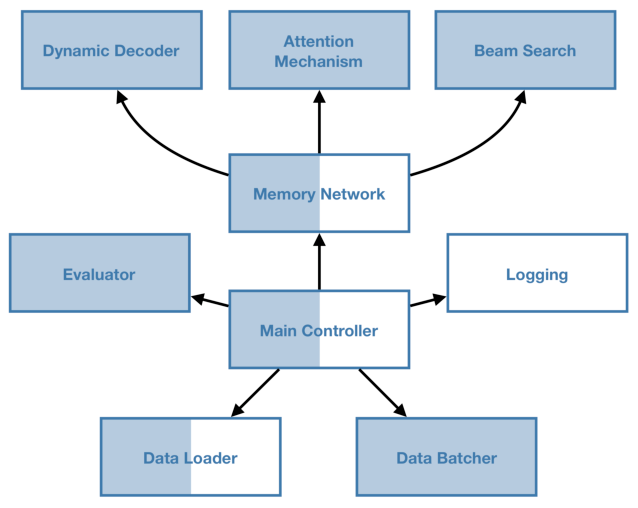
\includegraphics[scale=1.0]{assets/figures/components_orig.pdf}
\caption{(a) an example dialog with history and KB tuples. (b) an illustration of Mem2Seq memory. (c) an illustration of \sys\ memory}
\label{fig:sys_comp}
\end{figure}

\noindent\textbf{Main Controller}

\noindent\textbf{Data Loader}

\noindent\textbf{Data Batcher}

\noindent\textbf{Memory Network}

\noindent\textbf{Dynamic Decoder}

\noindent\textbf{Attention Mechanism}

\noindent\textbf{Beam Search}

\noindent\textbf{Evaluator}

\section{Parts of the \sys\-RL Architecture}

There are mainly three main components that have been added to the \sys\ architecture to make \sys -RL. These are listed below.

\begin{enumerate}
	\item \textbf{API Explorer} - T
	\item \textbf{Rewards} - 
	\item \textbf{RL-Decoder} - 
	\item \textbf{Augmented REINFORCE} - 
\end{enumerate}

We observe the interaction between these added components and the previous architecture in Figure \ref{fig:sys_comp_rl}.

\begin{figure}[t]
\centering
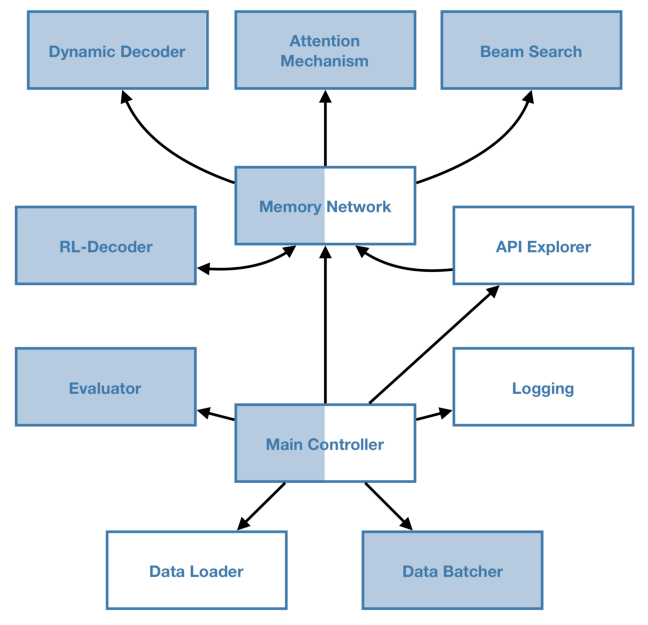
\includegraphics[scale=1.0]{assets/figures/components_rl.pdf}
\caption{(a) an example dialog with history and KB tuples. (b) an illustration of Mem2Seq memory. (c) an illustration of \sys\ memory}
\label{fig:sys_comp_rl}
\end{figure}

\noindent\textbf{Main Controller}

\noindent\textbf{Memory Network}
We added three main APIs in the memory network to enable the RL-decoder. The first, \emph{api\_predict} will attempt to predict good API responses via the RL-decoder policy and utilises beam search to get a large set predictions.

The second, \emph{api\_train} takes in APIs and their rewards and then implements the augmented REINFORCE algorithm

finally, the 

\noindent\textbf{RL-Decoder}

